%!TEX root =  ../main.tex

\chapterimage{amazing-736875_1280}
\mychapter{Infinities}{infinity}


In all of calculus, one number is unique, containing an infinite exponent in a finite number.
$e$ is hard to appreciate until you start considering rates of change, 
accumulated distance, or continuous growth.  

But what does infinity even mean?  Nothing in our world has even gone on without limit,
except perhaps black holes.  Aristotle said there are two kinds of infinities: potential and
actual.  But Georg Cantor said a physical potential infinity presupposes an actual infinity
in our minds, the mental construct we are saying would come into existence, if were to 
continue.

Amazingly, all this heady talk of math and philosophy has real-life implications.  The infinite
sum of all the natural numbers appears on page 22 of Joseph Polchinski's classic, 
\textit{String Theory}.  Calculus itself --- with all its myriad applications in our lives today
--- is the based on the assumption that a line is subdivided into a infinite number of
indivisible units.  Whether or not they exist in nature, infinities are useful mathematical
constructs.





\newpage
\chapterminitoc

%								8 - 1
\newpage
\section{e}
\subsection{Problems}
word doc
\newpage
%!TEX root =  ../main.tex


\subsection{Derivatives of Exponentials}


\objective{Describe and use the special status of $e^x$ amongst exponential equations}


As we move past power function, derivatives become a lot harder to compute.  If we
begin with the premise that there is some exponential function which is its own 
derivative --- that the height of the function at every point is the same as its slope
--- then we should find constant for the base.  Empirically, it is easy to see that
such a number is between 2 and 3, but how can we be more precise?  We
begin with the definition
$$
f'(x) = \lim_{h\rightarrow0}\frac{f(x+h)-f(x)}{h}
$$
We will use the letter $e$ next, but assume we do not know its exact value.  In
the problem set, you saw that it's definition is
$$
e = \lim_{h\rightarrow\infty}\left(1+\frac{1}{h}\right)^h
$$
and so right away we see we are dealing with opposite limits.  We can convert
from a limit at infinity to a limit at zero by taking the reciprocal of the variable
at every instance.  This leads to a modified definition of $e$:
$$
e = \lim_{h\rightarrow0}\left(1+\cfrac{1}{\frac{1}{h}}\right)^{\frac{1}{h}}
$$
Armed wth compatible limits, let us return to the definition of a derivative.
$$
(e^x)'  = \lim_{h\rightarrow0}\frac{e^{x+h}-e^x}{h}
$$
By the properties of exponents, a sum in the degree must come
from a multiplication of the bases (i.e. $e^{x+h}=e^x\cdot{}e^h$).
Factoring out $e^x$, we get
$$
(e^x)' = e^x \cdot{}\lim_{h\rightarrow0}\frac{e^h-1}{h}
$$
Will our definition of $e$ work here?  Substituting it in is very messy, but cleans up
perfectly.  Just evaluating the limit,
\begin{align*}
	\lim_{h\rightarrow0} & \frac{\left[\left(1+\cfrac{1}{\frac{1}{h}}\right)^{\frac{1}{h}}\right]-1}{h} &\\
	& \frac{1+\left(\cfrac{1}{\frac{1}{\frac{1}{h}}}\right) - 1}{h} &\\
	& \frac{\cfrac{1}{\frac{1}{h}}}{h} & \Rightarrow \frac{h}{h} \\
	& = 1
\end{align*}

\begin{derivation}{Derivative of $e^x$}
$$
(e^x)' = e^x
$$
\end{derivation}

\subsection{Implications}
How does this explain the behavior of $2^x, 3^x$ or any other base?  The limit portion of
the work shown above was equal to 1, but if we had substituted any other number in,
we would have obtained some constant.  We can extend the definition of exponential
derivative like so:

\begin{derivation}{Derivative of $b^x$}
$$
(b^x)' = b^x \cdot{} \ln{b}
$$
\end{derivation}

Often we will need to apply the Chain Rule, since the exponent is rarely just $x$
$$
\left(e^{f(x)}\right)' = e^{f(x)} \cdot f'(x)
$$

Lastly, if $e^x$ is it's own derivative, then it is its own anti-derivative as well:
$$
\int e^xdx = e^x + C
$$

The TI-8* has an $e^x$ function (2nd-LN) and most computer programs (e.g. MS Excel)
have a function \texttt{exp()}, which is the same thing.

\begin{figure}
\begin{centering}
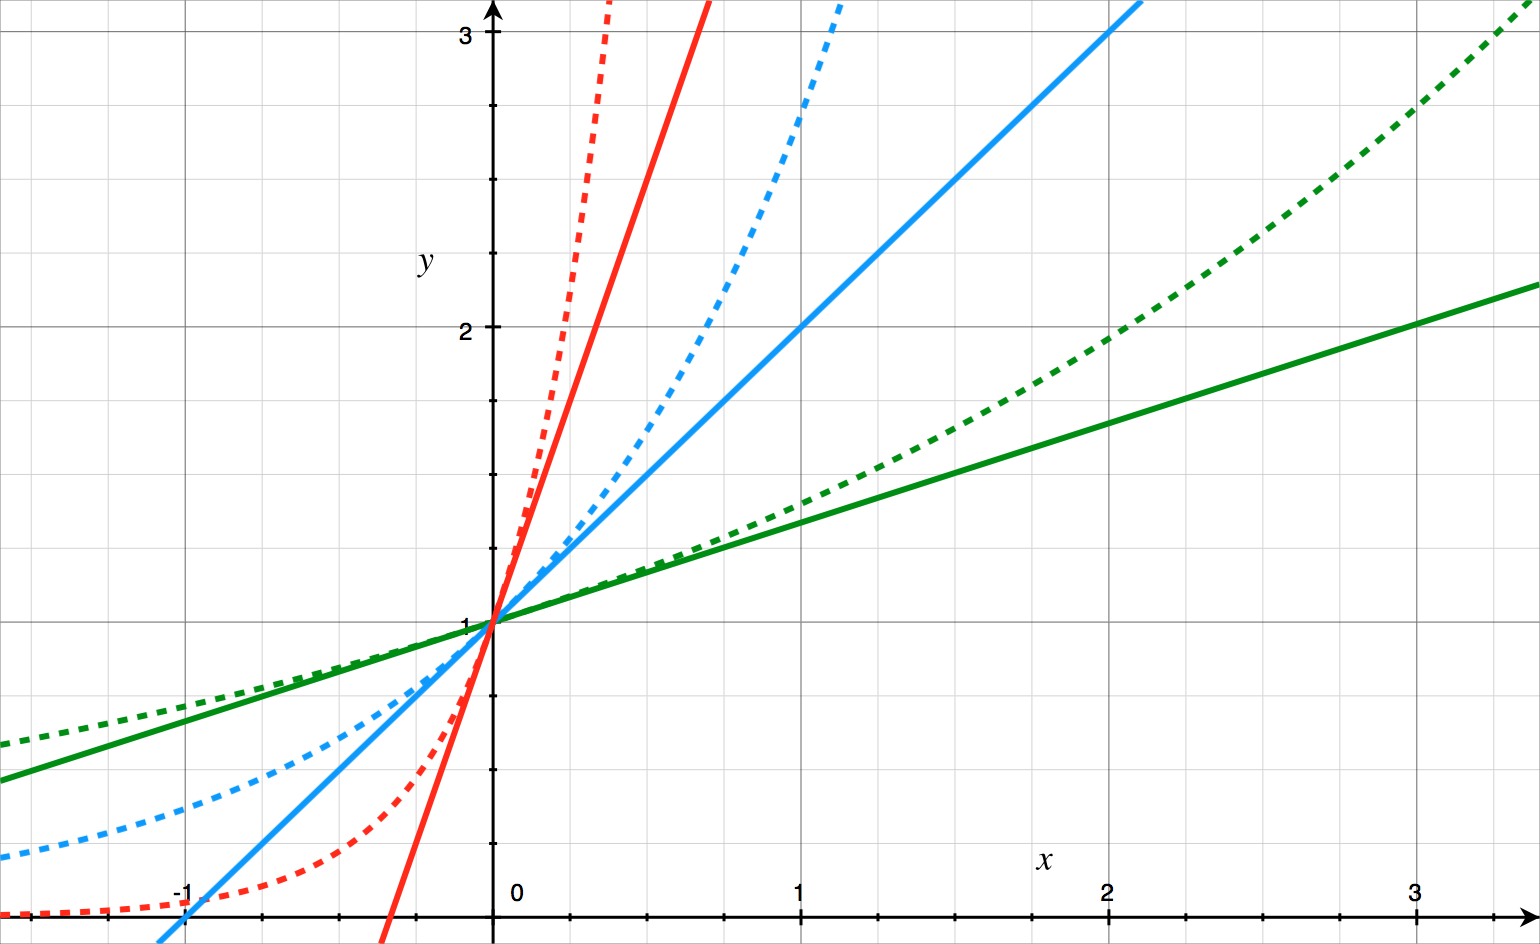
\includegraphics[width=\textwidth]{\chapdir/pics/exponentialderivatives}
\caption[Exponential tangent lines at (0,1)]{A set of exponential equations tangent lines at (0,1), with original function dotted.  $1.4^x$ in green, $e^x$ in blue, $20^x$ in red.}
\end{centering}
\end{figure}
\newpage
\subsection{Exercises}
Kuta and
Read chapter one --- ``Big Numbers'' --- of George Gamov's
\textit{One, Two, Three ... Infinity} .



%								8 - 2
\newpage
\section{Infinities}
\subsection{Problems}
Word doc
\newpage
%!TEX root =  ../main.tex

%https://numberwarrior.wordpress.com/2010/07/30/is-one-two-many-a-myth/
\begin{figure}
\begin{centering}
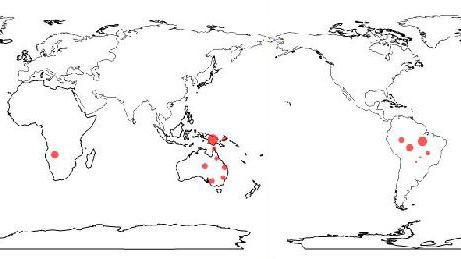
\includegraphics[scale=0.8]{\chapdir/pics/twocounting1}
\caption[Languages with only two numbers]{The number of languages with only the numbers ``1'' and ``2'' (i.e., ``3'' == ``many'') is very few, but not zero.}
\end{centering}
\end{figure}

\subsection{Matching}

\objective{Understand and apply definitions of $\aleph_0$ and $\aleph_1$ to hypothetical problems involving infinity.}

\subsection{Countable Infinity}
There are the same number of: natural numbers, even numbers, odd numbers, integers and
rational numbers.  That may seem difficult to believe (surely there are half as many even numbers
as whole numbers!), but it is demonstrable.  We cannot count to infinity (by definition) so,
according to Georg Cantor, we must \emph{match} or pair element from one set to another.
If there exists a partner for every element of one set in another, with none left over, then
we can say the sets are the same size, even if they are infinite.

\personfeature[-3in]{\chapdir/pics/Georg_Cantor3.jpg}{George Cantor}{1845-1918}{was a famous German mathematician, known for discovering and building a hierarchy of infinite sets according to their cardinal numbers. He is also known for inventing the Cantor set, which is now a fundamental theory in mathematics. Born into a family of musicians, he displayed an aptitude for music at a young age.
\href{https://en.wikipedia.org/wiki/Georg_Cantor}{Wikipedia}}

Now, consider the whole numbers, e.g. $0, 1, 2, 3, 4, \dots$.  While it would take an infinite 
amount of time to list them all (what Aristotle called a ``potential infinity'', meaning we can
conceive of how it potentially could be done), the whole numbers are conceivably countable,
so that infinity is called \textbf{countable infinity}.  Can we match the even up with them?
Yes!  Simply take each whole number, call it $n$, and map it onto $2n$, a unique even 
number.  This accounts for all of the whole numbers and all of the even numbers, so 
they are both countably infinite.  This infinity is called $\aleph_0$ (AL-eff NULL), because
it is the first infinity, and mathematicians start counting at zero.

It is each to see how the odds, the integers, and many other sets of numbers are also
of size $\aleph_0$, but things get trickier when we consider the rationals.  What does
your intuition tell you?  Cantor had to carefully construct a proof where he laid out 
all possible numerators in rows, and all possible denominators in columns.  By walking
diagonally through the list(s), he showed that it was possible to map the rationals
onto the wholes, and therefore they are the same size.

\begin{figure}[h]
\begin{centering}
\begin{tikzpicture}[myarrow/.style={red,->,shorten >=0.25cm, shorten <=.25cm}]
   \matrix (m) [draw,matrix of nodes,inner sep=.2cm,ampersand replacement=\&]
   {
    $\frac{1}{1}$ \& $\frac{1}{2}$ \& $\frac{1}{3}$ \& $\frac{1}{4}$ \& $\dots$\\
    $\frac{2}{1}$ \& $\frac{2}{2}$ \& $\frac{2}{3}$ \& $\frac{2}{4}$ \& $\dots$\\
    $\frac{3}{1}$ \& $\frac{3}{2}$ \& $\frac{3}{3}$ \& $\frac{3}{3}$ \& $\dots$\\
    $\frac{4}{1}$ \& $\frac{4}{2}$ \& $\frac{4}{3}$ \& $\frac{4}{4}$ \& $\dots$\\
    $\vdots$ \& $\vdots$ \& $\vdots$ \& $\vdots$ \& $\ddots$\\
   };
   \draw[myarrow] (m-1-1.center)--(m-2-1.center);
   \draw[myarrow] (m-2-1.center)--(m-1-2.center);
   \draw[myarrow] (m-1-2.center)--(m-1-3.center);
   \draw[myarrow] (m-1-3.center)--(m-2-2.center);
   \draw[myarrow] (m-2-2.center)--(m-3-1.center);
   \draw[myarrow] (m-3-1.center)--(m-4-1.center);
   \draw[myarrow] (m-4-1.center)--(m-3-2.center);
   \draw[myarrow] (m-3-2.center)--(m-2-3.center);
   \draw[myarrow] (m-2-3.center)--(m-1-4.center);
   \draw[myarrow] (m-1-4.center)--(m-2-4.center);
   \draw[myarrow,-,dotted] (m-2-4.center)--(m-3-3.center);
\end{tikzpicture}
\caption{Cantor's diagonal counting of the Rationals}
\end{centering}
\end{figure}

\subsection{Uncountable Infinity}
What about the irrational numbers?  Intuitively, you should see that there are more of
them, but intuition is not always trustworthy.  Every rational number is either a 
terminating or repeating decimal, but there can always be an infinity of irrationals
``in between'', with random digits.  Cantor employed another diagonal-type proof
in this case too, only now it will show a contradiction.

Suppose someone told you they had a list of all the irrational numbers, stored in 
some kind of crazy computer that could hold countably infinite number of numbers.
(A computer is convenient to bring into this story because computers store numbers
as 1's and 0's which makes this easier to demonstrate, but any list will do.)  Also
for simplicity's sake, let us just say we have listed all the irrationals from 0 to 1.
It is an infinite list of numbers, each with an infinite number of digits.


\begin{figure}
\begin{center}
  \begin{tabular}{ c | c c c c c c c c c  }
    \hline
    		& \textbf{0} & \textbf{1} & \textbf{2} & \textbf{3} & \textbf{4} & \textbf{5} & \textbf{6} & \textbf{7} & \textbf{8} \\ \hline 
    \textbf{0} & 0 & 1 & 0 & 1 & 0 & 0 & 0 & 1 & $\dots$ \\ 
    \textbf{1} & 1 & 1 & 1 & 0 & 1 & 0 & 1 & 1 & $\dots$ \\ 
    \textbf{2} & 1 & 0 & 0 & 1 & 1 & 1 & 1 & 0 & $\dots$ \\
    \textbf{3} & 0 & 1 & 1 & 0 & 0 & 1 & 0 & 0 & $\dots$ \\ 
    \textbf{4} & 1 & 0 & 1 & 0 & 0 & 1 & 0 & 1 & $\dots$ \\
    \textbf{5} & 0 & 1 & 1 & 1 & 0 & 0 & 0 & 0 & $\dots$ \\ 
    \textbf{6} & 1 & 1 & 0 & 0 & 0 & 1 & 1 & 0 & $\dots$ \\
    \textbf{7} & 0 & 1 & 0 & 1 & 0 & 0 & 0 & 1 & $\dots$ \\ 
    \textbf{8} & 0 & 0 & 1 & 0 & 0 & 0 & 0 & 0 & $\dots$ \\
    \textbf{9} & 1 & 1 & 0 & 1 & 0 & 1 & 0 & 1 & $\dots$ \\ 
    $\vdots$ & $\vdots$ & $\vdots$ & $\vdots$ & $\vdots$ & $\vdots$ & $\vdots$ & $\vdots$ & $\vdots$ & $\ddots$ \\
  \end{tabular}
\caption{A (supposed) list of all irrational binary numbers.}
\end{center}
\end{figure}

Now suppose I am a rather incorrigible bloke, and I come along an make a
number not on the list.  To do that, let us consider the main diagonal of the
list, i.e. coordinates (0,0, (1,1), (2,2), (3,3), etc.  Because this list in in binary 
(1's and 0's), it is very easy to make that place on my \emph{new} number
the opposite of whatever was on the list.  My new number is infinitely long, and
differs from every number on the original list in at least one decimal place, by
definition.  You might even add my number to the list, but I can do the same
process again and create a new number not on \emph{that} list.  I have
proven that the list of irrationals --- even just between 0 and 1 --- is \emph{not}
listable, and \textbf{uncountable infinity}.

The Reals, the Irrrationals, and other sets have a size we must notate as
$\aleph_1$ (AL-eff sub WUHN).





\newpage
\subsection{Exercises}
%\loadallproblems[0802]{ch08/0802x}
%\begin{multicols}{2}
%\renewcommand{\theenumi}{\thesection.\arabic{enumi}}
%\begin{enumerate}
%\foreachproblem[0802]{\item\label{prob:\thisproblemlabel}\thisproblem}
%\end{enumerate}
%\renewcommand{\theenumi}{\arabic{enumi}}
%\end{multicols}


%								8 - 3
\newpage
\section{Logarithmic Derivatives}
\subsection{Problems}
Word doc
\newpage
%!TEX root =  ../main.tex

\subsection{Deriving}

\objective{Prove the Power Rule, Product Rule, and Quotient Rule, and apply them to arbitrary derivatives}


Coming back to Earth for a section from all this contemplation of infinities, we see the
extreme usefulness of it all.  The number $e$ is not the answer to any algebraic 
expression.  That is, one cannot build a polynomial --- even an irregular one with
rational coefficients and rational exponents --- that has $e$ as a solution.  $e$ is a
transcendental number, the result of an infinite process, though it itself is a finite number.
There is a very important sense in which $e$ contains an infinity within itself.

It takes a system like calculus to create $e$, and it returns the favor by unleashing a
vast reservoir of new waters for calculus to navigate.  The derivative of $e^x$ is $e^x$,
and its inverse --- $\ln{x}$ --- is just as amazing.  The inverse of $y=e^x$ can be written
as $x=e^y$.  By implicit differentiation, $dx = e^ydy$, and therefore $\frac{dy}{dx} =
\frac{1}{e^x}$.  Well, we began by saying $e^y=x$, so the derivative of $\ln{x}$ must
be $\frac{1}{x}$.  Hopefully, you have been curious for several chapters what
could ever have the derivative of $\frac{1}{x}$, since nothing could ever make that
via the Power Rule.

\subsection{Proofs}
Speaking of the Power Rule, we have been using it as we made it via Induction for 
some time now.  Not that Induction is a bad thing, but ln affords us a more elegant 
proof.  Suppose $y$ is defined as some function to a power:
$$
y = \left(f(x)\right)^n
$$
There is no immediately obvious way to differentiate the left side of this identity, but
what if we take the log of both sides first?  This is called the \textbf{logarithmic deriviative}.
$$
\ln{y} = \ln{\left(f(x)\right)^n}
$$
A happy consequence comes from the fact that a log of a power is the same as the
log times the power.
$$
\ln{y} = n\cdot\ln{f(x)}
$$
Now we can take the derivative of both sides implicitly.
$$
\frac{1}{y} \cdot y' = n \cdot \frac{1}{f(x)}
$$
Solving for $y'$, we get
$$
y' = n \frac{y}{f(x)}
$$
If we substitute back in the original definition of $y$ (i.e. $\left(f(x)\right)^n$) and simplify,
we see
$$
y' = n\cdot{}\left(f(x)\right)^{n-1}
$$
the generalized Power Rule.


\subsection{Product and Quotient Rule}
The Product Rule can also be proven by Logarithmic Derivative, without limits, for any 
$y = f\cdot{}g$.
\begin{align*}
\ln{y} &= \ln{f \cdot{} g} \\
\frac{1}{y}y' &= \left(\ln(f)\right)' + \left(\ln(g)\right)' \\
y' &= y(\frac{1}{f}f' + \frac{1}{g}g') \\
 &= f\cdot{}g(\frac{1}{f}f' + \frac{1}{g}g') \\
 &= g\cdot{}f' + f\cdot{}g'
\end{align*}

The same goes for the Quotient Rule, for any $y=\frac{f}{g}$.
\begin{align*}
\ln{y} &= \ln{\frac{f}{g}} \\
\frac{1}{y}y' &= \left(\ln{f} - \ln{g}\right)' \\
y' &= y\left(\frac{1}{f}f' - \frac{1}{g}g'\right) \\
  &= \frac{f}{g}\left(\frac{f'}{f} - \frac{g'}{g}\right) \\
  &= \frac{f'}{g} - \frac{g\cdot{}f'}{g^2}\\
  &= \frac{g\cdot{}f' - g\cdot{}f'}{g^2}
\end{align*}


\subsection{Derivative Review}
Let us summarize all of the derivative shortcuts we have discerned.  You are 
responsible to prove without assistance all of these

We will use $u$ as a variable of differentiation because there might be a
(nested?) set of Chain Rules to apply before we get down to $x$.  Assuming
$u$ is a function of $x$:
\begin{equation}
\frac{d}{dx}u = u\cdot{}\frac{du}{dx}
\end{equation}

We have been given a looping cycle of trigonometric derivatives without proof:
\begin{equation}
\left(\sin{u}\right)' = \cos{u}\frac{du}{dx}
\end{equation}
\begin{equation}
\left(\cos{u}\right)' = -\sin{u}\frac{du}{dx}
\end{equation}
\begin{equation}
\left(-\sin{u}\right)' = -\cos{u}\frac{du}{dx}
\end{equation}
\begin{equation}
\left(-\cos{u}\right)' = \sin{u}\frac{du}{dx}
\end{equation}
Any polynomial or power function can be differentiated with the Power Rule:
\begin{equation}
\left(u^n\right)' = n\cdot{}u^{n-1}\frac{du}{dx}
\end{equation}
Any exponential function can be differentiated as follows:
\begin{equation}
(b^u)' = b^u\cdot{}\ln{u}\frac{du}{dx}
\end{equation}
Any logarithmic function can be differentiated as follows:
\begin{equation}
\left(\log_a{u}\right)' = \frac{1}{\ln{a}}\cdot{}\frac{1}{u}\cdot{}\frac{du}{dx}
\end{equation}

Together with the Product and Quotient Rule above, almost any major
function should be differentiable for you now.




\newpage
\subsection{Exercises}
Kuta


%								8 - 4
\newpage
\section{Dominance}
\subsection{Problems}
Word doc
\newpage
%!TEX root =  ../main.tex

\subsection{Indeterminate Forms}

\objective{Classify difficult limits problems and solve via certain techniques}


Just as we used limits to define the derive six chapters ago, now they return the favor
and derivatives themselves allow us to find certain limits.  We have seen how removable
discontinuities take the form $\frac{0}{0}$, but what are we to do if a derivative
produce that form?  In fact, there are many forms which mathematicians classify
as \textbf{indeterminate}

$$
\frac{0}{0} , \frac{\infty}{\infty} , 0\times\infty , \infty-\infty , 0^0 , ^\infty \text{, and } \infty^0 
$$

These are all indicative of a variety of answers, some finite, some infinite.  There is
no way to know what answer will predominate in the end without more work.
Consider this limit
\begin{equation}
\lim_{x\rightarrow0}\frac{5x}{\ln(x+1)}
\end{equation}
Obviously, if we attempt a direct evaluation, we get a meaningless answer.  But
consider what we know about this quotient function.  Every ``nudge'' in the $x$
direction (dx) will produce a small change in the top half of the fraction: 5dx, to
be precise.  Similarly, the change in the denominator (it's implicit differential)
is $\frac{1}{x+1}$dx.  As a fraction, this is $\cfrac{5dx}{\frac{1}{x+1}dx}$ or 
$5(x+1)$.  Notice this is not like the maneuvering we did with removable 
discontinuities; we have not constructed an identical but hole-less version
of the equation.  Our new equation is useful because it goes through the hole.


This technique for solving limits at indeterminate value is call \textbf{L'Hopital's}
Rule (LO-pee-talz), even though it was found by L'Hopital's collegue Bernoulli.

\subsection{Infinite Forms}
Not every form with a zero in the denominator or an infinity in it is indeterminate.
The following forms resolve in other ways, and cannot be solved with L'Hopital's
Rule:
$$
\frac{1}{0} , \frac{\infty}{1} , \frac{\infty}{0} , \infty + \infty , \infty \times\infty
$$

Some other fractions you should recognize from algebra and/or experience as zero:
$$
\frac{0}{1} = \frac{1}{\infty} = \frac{0}{\infty}
$$

To return to our earlier equation of $\frac{5x}{\ln(x+1)}$, what is the limit as $x$ 
approaches infinity?  Logarithmic graphs \emph{seem} to taper off, and direct 
evaluation is useless (plugging in infinity for $x$) because we get $\frac{\infty}{\infty}$.
But L'Hopital's Rule works here too, because that is an indeterminate form.
Our limit will be the same as 
\begin{equation}
\lim_{x\rightarrow0}5(x+1)
\end{equation}
which is infinite.
\newpage
\subsection{Exercises}
in Kuta


%								8 - 5
\newpage
\section{Analyses}
\subsection{Problems}
Word
\newpage
%!TEX root =  ../main.tex

\subsection{Real Analysis}

\objective{Apply the basic principles of Analysis to solve improper integral and use hyperreal numbers}


An \textbf{improper integral} is a definite limit where one and/or the other bound is
an infinity.  For example, 
$$
\int_0^\infty e^{-x}dx
$$
In this case, we integrate like normal, but take the upper bound to be a limit, 
written more simply.  (No one wanted to write a limit on top of an integral!)  
$$
\int_0^\infty e^{-x}dx = \left.-e^{-x}\right|_0^\infty = \lim_{x\rightarrow\infty} -e^{-x} - -e^0
$$
The limit approaches 0 while the function evaluates to -1.  We say, therefore, that
the entire integral is assigned a value of 1.  What are we saying?  The area under
an infinite curve is a finite number?  Remarkable.

\subsubsection{Special Functions}
Some functions come up so often in higher mathematics that they are given
their own name, often involving Greek letters.  Many of them have wildly 
complicated definitions, and not a few are improper integrals.  One such
function is the Gamma function, which is defined thus:

\begin{equation}
\Gamma(z)=\int_{0}^{\infty}x^{z-1}e^{-x}dx
\end{equation}

We shall see in chapter 14 that there is very common function in math called
\textbf{factorial}.  The Gamma function is the \textbf{analytic continuation} of
the factorial function, such that $\Gamma(n) = (n-1)!$.  This has many uses in
probability theory, allowing us to calculate values in between the integers.


\subsection{Non-Standard Analysis}
When Leibniz and Newton invented Calculus in the mid-17th century, their discoveries were
a culmination of two centuries of fierce debate over the idea of infinitesimals.  Was the
continuum (we might use the were ``number line'' or Reals) made up on indivisible, smallest
elements or not?  Leibniz called the infinitesimals and Newton called them fluxions.  
The assumption of their existence had made it possible to grow beyond a dependence
upon Euclid and the Classics, and enabled the ability to make new discoveries in 
mathematics, along the lines of Analytic Geometry (the algebra of Geometry).


Unfortunately, Newton and Leibniz did not cultivate a rigor science of infinitesimals,
and later centuries have much preferred the work of Cauchy and Weierstrauss, 
because of its consistency and explanatory power.  However, given the antiquity of
the method of \textbf{exhaustion} and current understand of Planck Length, 
Planck Time, Planck Mass, etc., this textbook has attempted to keep some measure
of the method of infinitesimals at its core.  These methods were made rigorous in
the 1960s by Abraham Robinson and codified in a system of numbers known as 
\textbf{Hyperreal} Numbers, or simply, the Hyperreals.

The hyperreals are an extension of the reals, as the name implies.  We need only
posit two numbers: $\omega$ and $\epsilon$.  $\omega$ (the last letter of the
Greek alphabet, only always lowercase, pronounced oh-MEG-uh or oh-MAY-guh)
is analogous to infinity as most people think of it.  Infinity is \emph{supposed}
to be a concept, not a number, the idea of going on without end.  $\omega$ is
a number bigger than any real number, just smaller than infinity.  $\epsilon$ is
its reciprocal, a positive number smaller than any real number but not zero.

This leads to a system where numbers may be composed of two (even three)
parts.  For example, $3+2\epsilon$ may not be simplified any further.  But 
$\omega(3+2\epsilon)$ can be: $3\omega + 2$.  What good is such an arbitrary,
new system.  Well actually, its quite old and caused the invention of calculus!

\subsubsection{Old Definitions}
The Difference Quotient can be stated without limits using hyperreals as
\begin{equation}
f'(x) = \frac{f(x+\epsilon) - f(x)}{x+\epsilon -x}  \outnote{(Hyperreal Difference Quotient)}
\end{equation}

$e$ can be stated without limits as follows:
\begin{equation}
e = (1+\epsilon)^\omega  \outnote{(Hyperreal Definition of $e$)}
\end{equation}

\subsubsection{Derivative}
Let us do one example, with several others in the exercises, finding the derivative of 
$x^2$.
$$
(x^2)' = \frac{(x+\epsilon)^2-x^2}{\epsilon} = \frac{x^2+2x\epsilon+\epsilon^2-x^2}{\epsilon}
= 2x+\epsilon
$$
Unlike limits notation, the infinitesimal does not disappear.  Every $\epsilon$ step in
the $x$-direction produces a jump of $2x$ in the $y$-direction.  According to quantum
mechanics (and Zeno's Paradox), the jumps are done without intervening steps,
that at the smallest level, elementary particles proceed in a way quite unlike
our macroscopic world.

\newpage
\subsection{Exercises}
In kuta




%								8 - 6
\newpage
\section{Review}
\subsection{Chapter Review}
\subsection{Chapter Test}
\subsection{Cumulative Review}
This unit has been a diverse whirlwind.  We united almost everything we had ever seen
before in math where $x$ had an exponent on it under the heading ``Power Function''.
Next we added such things together to get polynomials.  Then we divided those by each
other and got rational functions.  Then we swapped where $x$ was and put it in the
exponent.  This produced functions which ``transcended'' algebra, where ordinary inputs
could produce amazingly irrational answers.  The inverses of these functions were called
logs.

This transcendental leap allowed us to get a perspective on mathematics itself.  What 
are we doing here?  Are all these abstract things just in our minds?  If so, why do they 
works so well in the world?  It is surprisingly easy to imagine some things that 
seemingly do not exist: namely infinities.  Some are countable, some are not.  Such
crazy ideas were necessary to continue finding derivatives to everything kind of function
we might need in the world, but they produce some logical conundrums.   But they
are the very foundation of all the calculus we have been doing!

in the world
\subsection{Cumulative Test}